\documentclass[tikz,border=6pt]{standalone}
\usepackage{fontspec}
\setmainfont{Linux Libertine O}
\usetikzlibrary{calc}
\definecolor{udcblue}{HTML}{1f77b4}
\definecolor{udcpink}{HTML}{c23b75}
\definecolor{udcorange}{HTML}{d97927}
\definecolor{udcgreen}{HTML}{3f8f3f}
\definecolor{udcteal}{HTML}{2a8c8c}
\begin{document}
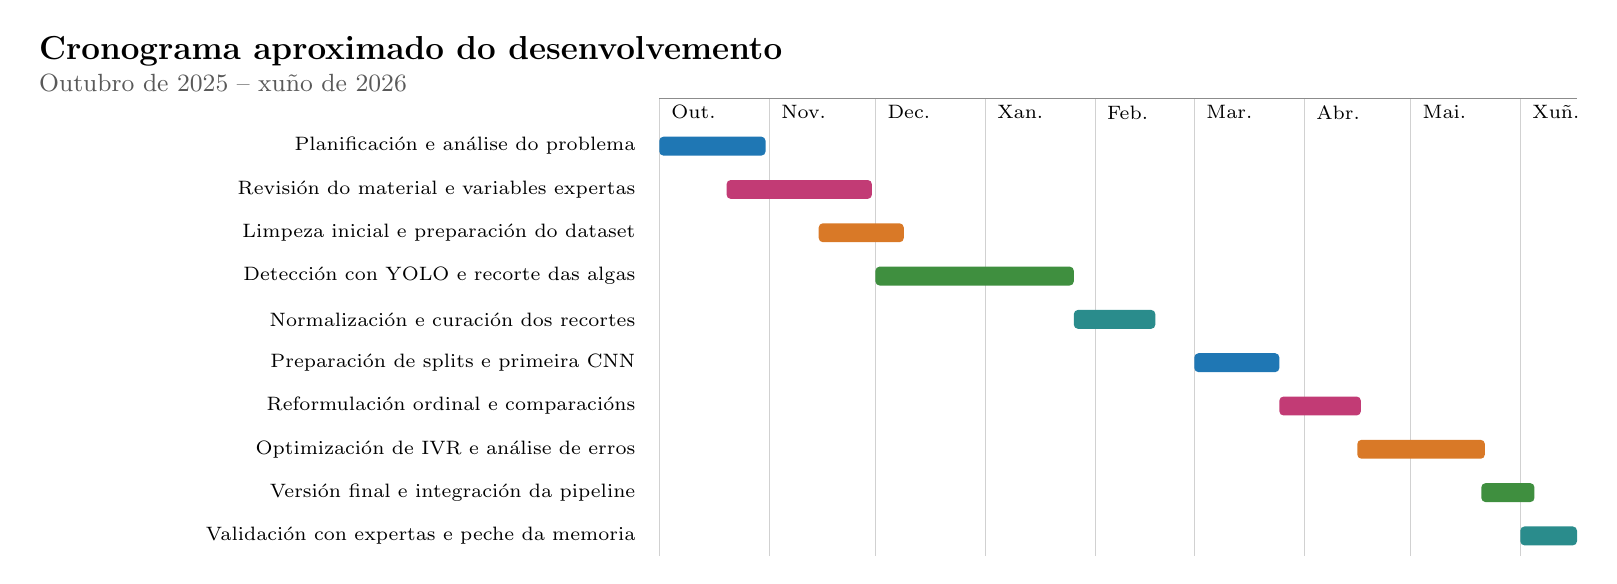
\begin{tikzpicture}[x=1cm,y=1cm]
\node[anchor=west,font=\bfseries\large] at (-8.0,0.65) {Cronograma aproximado do desenvolvemento};
\node[anchor=west,font=\small,text=black!65] at (-8.0,0.25) {Outubro de 2025 -- xuño de 2026};
\draw[black!18] (0.000,0.05) -- (0.000,-5.750);
\node[anchor=west,font=\scriptsize] at (0.030,-0.12) {Out.};
\draw[black!18] (1.395,0.05) -- (1.395,-5.750);
\node[anchor=west,font=\scriptsize] at (1.425,-0.12) {Nov.};
\draw[black!18] (2.745,0.05) -- (2.745,-5.750);
\node[anchor=west,font=\scriptsize] at (2.775,-0.12) {Dec.};
\draw[black!18] (4.140,0.05) -- (4.140,-5.750);
\node[anchor=west,font=\scriptsize] at (4.170,-0.12) {Xan.};
\draw[black!18] (5.535,0.05) -- (5.535,-5.750);
\node[anchor=west,font=\scriptsize] at (5.565,-0.12) {Feb.};
\draw[black!18] (6.795,0.05) -- (6.795,-5.750);
\node[anchor=west,font=\scriptsize] at (6.825,-0.12) {Mar.};
\draw[black!18] (8.190,0.05) -- (8.190,-5.750);
\node[anchor=west,font=\scriptsize] at (8.220,-0.12) {Abr.};
\draw[black!18] (9.540,0.05) -- (9.540,-5.750);
\node[anchor=west,font=\scriptsize] at (9.570,-0.12) {Mai.};
\draw[black!18] (10.935,0.05) -- (10.935,-5.750);
\node[anchor=west,font=\scriptsize] at (10.965,-0.12) {Xuñ.};
\draw[black!45] (0,0.05) -- (11.655,0.05);
\node[anchor=east,font=\scriptsize,align=right,text width=7.6cm] at (-0.18,-0.550) {Planificación e análise do problema};
\fill[udcblue,rounded corners=1.5pt] (0.000,-0.670) rectangle (1.350,-0.430);
\node[anchor=east,font=\scriptsize,align=right,text width=7.6cm] at (-0.18,-1.100) {Revisión do material e variables expertas};
\fill[udcpink,rounded corners=1.5pt] (0.855,-1.220) rectangle (2.700,-0.980);
\node[anchor=east,font=\scriptsize,align=right,text width=7.6cm] at (-0.18,-1.650) {Limpeza inicial e preparación do dataset};
\fill[udcorange,rounded corners=1.5pt] (2.025,-1.770) rectangle (3.105,-1.530);
\node[anchor=east,font=\scriptsize,align=right,text width=7.6cm] at (-0.18,-2.200) {Detección con YOLO e recorte das algas};
\fill[udcgreen,rounded corners=1.5pt] (2.745,-2.320) rectangle (5.265,-2.080);
\node[anchor=east,font=\scriptsize,align=right,text width=7.6cm] at (-0.18,-2.750) {Normalización e curación dos recortes};
\fill[udcteal,rounded corners=1.5pt] (5.265,-2.870) rectangle (6.300,-2.630);
\node[anchor=east,font=\scriptsize,align=right,text width=7.6cm] at (-0.18,-3.300) {Preparación de splits e primeira CNN};
\fill[udcblue,rounded corners=1.5pt] (6.795,-3.420) rectangle (7.875,-3.180);
\node[anchor=east,font=\scriptsize,align=right,text width=7.6cm] at (-0.18,-3.850) {Reformulación ordinal e comparacións};
\fill[udcpink,rounded corners=1.5pt] (7.875,-3.970) rectangle (8.910,-3.730);
\node[anchor=east,font=\scriptsize,align=right,text width=7.6cm] at (-0.18,-4.400) {Optimización de IVR e análise de erros};
\fill[udcorange,rounded corners=1.5pt] (8.865,-4.520) rectangle (10.485,-4.280);
\node[anchor=east,font=\scriptsize,align=right,text width=7.6cm] at (-0.18,-4.950) {Versión final e integración da pipeline};
\fill[udcgreen,rounded corners=1.5pt] (10.440,-5.070) rectangle (11.115,-4.830);
\node[anchor=east,font=\scriptsize,align=right,text width=7.6cm] at (-0.18,-5.500) {Validación con expertas e peche da memoria};
\fill[udcteal,rounded corners=1.5pt] (10.935,-5.620) rectangle (11.655,-5.380);
\end{tikzpicture}
\end{document}
